\documentclass[reprint,amsmath,amssymb,aps]{revtex4-1}
\usepackage[spanish,es-tabla]{babel}
\usepackage[utf8]{inputenc}
\usepackage{graphicx}
\usepackage{dcolumn}
\usepackage{bm}
\usepackage{amsmath}
\usepackage{bigints}
\usepackage{gensymb}
\usepackage{mathrsfs}
\usepackage[T1]{fontenc}
\usepackage[none]{hyphenat}
\usepackage{booktabs}
\usepackage[normalem]{ulem}
\usepackage{soul}
\useunder{\uline}{\ul}{}
\usepackage[table,xcdraw]{xcolor}
\usepackage{newunicodechar}
\usepackage{enumerate}
\usepackage{hyperref}
\usepackage[maxbibnames=99, sorting=none, backend=biber]{biblatex}
\addbibresource{biblio.bib}
\renewcommand\thesection{\arabic{section}}
\renewcommand{\tablename}{TABLA}
\newunicodechar{°}{\degree}
\usepackage{float}
\usepackage{etoolbox}
\makeatletter
\patchcmd{\frontmatter@RRAP@format}{(}{}{}{}
\patchcmd{\frontmatter@RRAP@format}{)}{}{}{}
\renewcommand\Dated@name{}
\makeatother


\begin{document}
\footnotesize
\preprint{APS/123-QED}

\title{Proyecto Astrofísica Computacional 1}

\author{\large Eduardo Andres Delgadillo Monsalve, Iván Gabriel Mafla Bolaños, Nicola Sebastián Miranda Niño}
 \affiliation{\texttt{eadelgadillom@unal.edu.co,}\texttt{imafla@unal.edu.co,}\texttt{nsmirandan@unal.edu.co}\\
 \normalsize { Universidad Nacional de Colombia, Sede Bogotá. 18 de Octubre del 2023}
 }
\begin{abstract}
\normalsize
\begin{center}\textbf{Resumen}\\
El presente artículo describe un proyecto de crossmatching entre dos catálogos astronómicos, a saber, el catálogo de radio AT20G y el catálogo óptico SuperCosmos. Se aplicaron varios algoritmos de machine learning, incluyendo Support Vector Machines (SVMs), Regresión Logística, Redes Neuronales y Redes Neuronales Convolucionales, con el objetivo de identificar y asociar objetos celestes en ambos catálogos. Se realizó un procesamiento inicial de los datos, que transformó el problema de identificación y correlación de objetos en uno de clasificación binaria. Cada uno de estos algoritmos fue evaluado en términos de precisión y rendimiento. Los resultados obtenidos de cada uno de los algoritmos fueron combinados para determinar las coincidencias entre los catálogos. En general, se encontró que todos los algoritmos alcanzaron una precisión superior al 95\%. El estudio se centró en un conjunto de 320 objetos del catálogo AT20G, de los cuales 91 no tenían coincidencias previamente identificadas en el catálogo SuperCosmos. Con la aplicación de los algoritmos de crossmatching, se lograron identificar un total de 78 nuevas coincidencias entre estos objetos, lo que representa un avance significativo en la comprensión de la distribución de objetos celestes en ambos catálogos. 
 
\end{center}
\textbf{Palabras Clave: Crossmatching, AT20G, SuperCosmos, SVM, Regresión Logística, Redes Neuronales, CNN} . 
\end{abstract}
\maketitle

\section{Introducción}

En la actualidad el crossmatching es cada vez más importante en la astronomía multimensajero (entendida como la astronomía que se puede realizar con información de distintas fuentes) ya que provee información adicional a la obtenida teniendo en cuenta una única fuente de información. Un objeto que se detecta en múltiples longitudes de onda ofrece más parámetros que podrían ser usados en su clasificación. Por ejemplo, una galaxia con fuertes emisiones tanto en el óptico como en el radio podría ser un candidato para ser una galaxia con un núcleo activo (AGN). Además, algunos tipos de objetos solo se pueden confirmar mediante observaciones en múltiples longitudes de onda como los blazares que son una clase de AGN que son muy brillantes en el radio y en el óptico, especialmente.

Teniendo en cuenta lo anterior, el presente trabajo presenta un crossmatching entre el catálogo AT20G \cite{AT20G}, el cual capta señales de radio a 20 GHz, y el catálogo Supercosmos \cite{Super} que capta señales en el óptico. Para ello, se aplicaron diferentes algoritmos de machine learning entre los que se encuentran el SVM (Support Vector Machine), la regresión logística y las redes neuronales \cite{ML}, los cuales se entrenaron con las coincidencias que ya se encontraban en el catálogo de radio  y se aplicaron para predecir las coincidencias de los objetos en radio que no se habían relacionado con los objetos descritos en el óptico.
Además, considerando que, uno de los parámetros relevantes que determinan las coincidencias actuales en el catálogo de radio con el de SuperCosmos es la magnitud en B, y, que alrededor de 46 objetos del AT20G no disponían del valor de este parámetro, se entrenó también una CNN usando las imágenes FITS en el filtro B de los objetos de radio con coincidencia en SuperCosmos. De esta forma, se intenta predecir la magnitud B de los objetos que permitiría completar este parámetro en el AT20G y verificar el valor predicho con la CNN con el valor obtenido en el crossmatching. 

\section{Metodología}
En la presente sección se describirá el procedimiento que se realizó para construir la base de datos que fue utilizada para el entrenamiento de los algoritmos de machine learning, así como, el procedimiento que se utilizó para aplicar dichos algoritmos para determinar las coincidencias entre el catálogo en radio y el catálogo en óptico.  
\subsection{Datos}
Previamente a aplicar cualquier algoritmo de machine learning, fue necesario crear una base de datos que permitiera entender el problema de crossmatching como un problema de clasificación binaria. Para ello, se realizó una unión entre el catálogo en radio y el catálogo en óptico, donde por cada objeto identificado en radio se encontraban varios objetos en el óptico contenidos en un radio o área de búsqueda que corresponde a la incertidumbre en la posición de los objetos detectados en radio,la cual era superior a la de los detectados en el óptico. De esta manera se obtuvo un conjunto de datos con un total de 2987 registros. Este conjunto inicial de datos se redujo al suprimir objetos que no poseían los valores completos, en los parámetros de interés. Esto se debe principalmente a errores en medición, mediciones que no aplican al objeto o valores que se desbordan de los límites habituales. Después de realizar este proceso se obtuvo una base de datos compuesta por 1207 registros, donde las características físicas que se tomaron en cuenta, considerando lo mencionado \cite{ML}, son las enunciadas en la tabla \ref{tab:my_label}.

\begin{table}
    \centering
    \begin{tabular}{|c|c|} \hline
    \rowcolor[HTML]{EFEFEF}
         Característica Física & Catálogo \\ \hline
         Densidad de Flujo a 20 GHz & AT20G \\ \hline
         Redshift & AT20G  \\ \hline
         Flujo Integrado a 20 GHz& AT20G \\ \hline
         Separación & AT20G-Supercosmos \\ \hline
         Magnitud en B& Supercosmos \\ \hline
         B-R& Supercosmos \\ \hline
         B-I& Supercosmos \\ \hline 
         Elipticidad en B& Supercosmos \\ \hline
    \end{tabular}
    \caption{Variables físicas utilizadas en la base de datos de clasificación por catálogo. Nótese que la variable separación corresponde a la distancia que existe entre las coordenadas en el catálogo de radio y en el óptico.}
    \label{tab:my_label}
\end{table}
Ahora bien, para aplicar algoritmos de aprendizaje supervisado es necesario que los datos tengan una etiqueta por lo cual el catálogo en radio debía tener un conjunto de objetos que ya se hubieran relacionado con un objeto en el óptico. Esta fue la razón por la que entre los distintos catálogos en radio se escogió el AT20G, pues este presentaba para algunos objetos el valor de la magnitud en el filtro B que fue extraída del Supercosmos lo que permitió crear una columna adicional a las enunciadas en la tabla \ref{tab:my_label}, nombrada "Coincidencia" donde se etiquetó la coincidencia entre objetos con un valor de ``1'' y las que no correspondían con ``0''. Ahora bien, no todos los objetos del AT20G reportaban la magnitud en B por lo cual estos objetos fueron extraídos de la base de datos de entrenamiento y se localizaron en una base datos de prueba, a la cual posteriormente se le aplicó los modelos de machine learning entrenados para determinar si presentaban coincidencias con alguno de los objetos en el óptico.

De esta manera, fue posible crear una base de datos de 760 datos etiquetados, esto es para cada objeto en radio se determinó su coincidencia en el óptico que se identificó con ``1'' y objetos próximos a su ubicación que no se identificaron con dicho objeto y por lo cual su valor de coincidencia era ``0''. Así mismo, se creó una base de datos de predicción compuesta de 447 datos, donde para cada objeto en radio se encontraban asociados distintos objetos en el óptico que se encuentran en posiciones próximas a la localización que para éste se reporta en el AT20G.


\subsection{Métodos de Machine Learning}
Una vez creada la base de datos de entrenamiento se entrenaron con ella algoritmos de machine learning como el SVM (Support Vector Machine), la regresión logística y la red neuronal. Sin embargo, debido a que las variables de flujo integrado y redshift no se encontraban completas para todos los objetos en el catálogo de radio fue necesario realizar varios entrenamientos cambiando el conjunto de entrenamiento. De esta manera, se crearon distintos modelos, a saber:
\begin{itemize}
\item Conjunto de modelos A: En este caso se entrenaron los algoritmos con todas las variables descritas en la tabla \ref{tab:my_label}. El número de datos del conjunto de entrenamiento fue de 405 y en el de predicción de 157.
\item Conjunto de modelos B: En este caso se entrenaron con todas las variables descritas en la tabla \ref{tab:my_label} a excepción del redshift. El número de datos en el conjunto de entrenamiento fue de 621 y en el de predicción de 297.
\item Conjunto de modelos C: En este caso se entrenaron con las variables descritas en la tabla \ref{tab:my_label} sin tener en cuenta el redshift y el flujo integrado. El número de datos en el conjunto de entrenamiento fue de 760 y en el de predicción de 447.
\end{itemize}

\subsubsection{SVM (Support Vector Machine)}
En el caso del algoritmo SVM se crearon cuatro modelos en los cuales se utilizaron los kernel ``Linear'' (lineal), ``rbf'' ( Radial Basis Funtion) con $\gamma=1$ y ``poly''(Polinomial) de grado 2 y 3. Así mismo, para el entrenamiento de cada modelo se aplicó un modelo de validación cruzada k-fold con k=10, siguiendo el procedimiento que se estableció en \cite{ML}. 
\subsubsection{Regresión Logística}
En el desarrollo del proyecto se aplicó también un algoritmo de regresión logística debido a la naturaleza de clasificación binaria con la que se analizó el problema de crossmatching. Se trata de una una función sigmoide que permite modelar la probabilidad de que una observación pertenezca a una de las clases en este caso de que se trate o no de una coincidencia. La descripción general del algoritmo implementado es la siguiente. 
Se creó un objeto de regresión logística utilizando la clase LogisticRegression del módulo sklearn (linear model). Se especificó el parámetro solver como "liblinear", que es un algoritmo de optimización adecuado para el problema de clasificación binaria. Luego se entrenó el modelo sobre los conjuntos de entrenamiento "X" (escalados previamente) y "y" tomando el número de parámetros correspondientes a cada conjunto de modelos A, B o C. Se evaluó el modelo sobre los conjuntos de prueba utilizando la métrica "Validation Score". 

\subsubsection{Redes Neuronales}
De igual manera, para cada conjunto de modelos se entrenaron diferentes esquemas de redes neuronales determinando las dos que presentaron los mejores resultados con la estructura más simple posible. Para tener una mejor precisión en los resultados de las redes neuronales en la capacidad de generalización de las predicciones se utilizó validación cruzada 10-fold.
\paragraph{Red neuronal esquema 1}
Para la primera red neuronal se utilizó el siguiente esquema secuencial:
\begin{itemize}
\item Capa de entrada densa con 12 neuronas en el Modelo A, 11 en el B y 10 en el C.  Esto, en función del número de parámetros usados en cada conjunto de acuerdo a lo descrito en la sección B.
\item Capa oculta densa con 16 neuronas y función de activación ReLU.
\item Capa oculta densa con 16 neuronas y función de activación ReLU.
\item Capa de salida densa con 2 neuronas y función de activación Softmax ya que se trata de un modelo de clasificación binaria. La función Softmax produce una distribución de probabilidad sobre las clases de salida, en este caso dos "0" y "1".

Se utilizó optimizador Adam, función de pérdida Sparse Categorical Crossentropy para las dos clases con valores enteros de clasificación binaria y métrica de rendimiento de la red de precisión. Se escalaron los valores de "X", y se entrenó la red con los conjuntos de entrenamiento de "X" y "y" con 1000 épocas. Finalmente, se evaluó la red con la métrica de precisión sobre los conjuntos de prueba y se realizaron las predicciones sobre el conjunto de predicciones.
\end{itemize}
\paragraph{Red neuronal esquema 2}
Para la segunda red se utilizó el siguiente esquema secuencial:
\begin{itemize}
\item Primera capa densa con 64 neuronas y función de activación ReLU, con entrada de la forma de X que corresponde al número de parámetros usados para el entrenamiento, 12, 11 y 10 según el conjunto de modelos utilizado.
\item Segunda capa densa con 32 neuronas y función de activación ReLU.
\item Tercera capa con 16 neuronas y función de activación ReLU.
\item Capa de salida con una sola neurona, a diferencia de la red con esquema 1, pero con con función de activación Sigmoide. Esta función produce una salida en el rango entre 0 y 1, que, así mismo, se interpreta como la probabilidad de tener una coincidencia.

Se utilizó optimizador Adam, función de pérdida Binary Crossentropy, adecuada para clasificación binaria y métrica de precisión para la evaluación de la red. El entrenamiento y evaluación se realizó sobre los conjuntos de entrenamiento de "X" (escalados previamente) y "y" utilizando entre 50 y 100 épocas y batch size de 32 para acelerar el proceso. En este caso, se utilizó además, un conjunto de validación durante el entrenamiento. Finalmente, se evaluó la red y se realizaron las predicciones de forma similar a la red con esquema 1.
\end{itemize}

\subsubsection{Red Neuronal Convolucional}
Se entrenó una red neuronal convolucional para predecir la magnitud en B de los objetos del catálogo AT20G. Se utilizaron las imágenes en el filtro B obtenidas en el catálogo de SuperCosmos para los objetos que registraban coincidencia en el AT20G. Aunque el número de imágenes disponibles es reducido para este tipo de problemas se logró predecir este valor de manera aceptable. Creados el archivo con las imágenes FITS de los objetos, que posteriormente fueron normalizadas, y el arreglo de numpy con la etiquetas de las magnitudes en B se implementó la siguiente estructura secuencial de la CNN:
\begin{itemize} 
    \item Primera capa convolucional con 64 kernels de tamaño 3x3, función de activación ReLU, con imágenes de 80x80 pixeles en un solo canal (escala de grises).
    \item Segunda capa MaxPooling de agrupación máxima 2x2 para disminuir la resolución de las características y disminuir el número de parámetros.
    \item Tercera capa convolucional con 64 filtros de 3x3 y función de activación ReLU.
    \item Cuarta capa MaxPooling de 2x2.
    \item Quinta capa Flatten para aplanar las características en un vector unidimensional para que se puedan conectar a las capas densas de la red.
    \item Sexta capa densa con 64 neuronas y función de activación ReLU.
    \item Capa de salida densa con una sola neurona y sin función de activación específica ya que se está realizando una regresión que produce una única salida numérica de la magnitud en B.
\end{itemize}
Todas las capas convolucionales utilizaron el parámetro "padding" igual a "same" para mantener el tamaño original de las entradas a la capa.
Se entrenó la red sobre los conjuntos de entrenamiento de imágenes y etiquetas por 30 épocas y batch size de 32. Se realizó la evaluación del modelo con la métrica del error cuadrático medio (mse). 

\section{Análisis y Resultados} 
\subsection{SVM (Support Vector Machine)}
Como se mencionó en la sección anterior cada algoritmo de aprendizaje supervisado se entrenó con varios conjuntos de entrenamiento que permitieron agrupar los distintos algoritmos en los grupos A, B y C, cuyos resultados se expresan en las siguientes secciones.
\subsubsection{Modelos A}
Al entrenar el algoritmo SVM con la base de datos descrita en la sección anterior y aplicar un modelos de validación cruzada fue posible obtener las matrices de confusión promedio para el conjunto de prueba que se ilustran en las figuras \ref{fig:1}, \ref{fig:2}, \ref{fig:3} y \ref{fig:4}. En este caso es relevante mencionar que para realizar el k-fold se utilizó la función de scikit learn \texttt{StratifiedKFold}, la cual permitía crear conjuntos de entrenamiento y prueba que conservaran los porcentajes de las variables binarias de la columna ``Coincidencia'' de la base de datos. Esto es importante debido a que existe una mayor cantidad de ``0'' que de ``1'' puesto que para un objeto en el catálogo de radio existen varios en el óptico dentro del radio de búsqueda, donde solo uno de estos es una coincidencia.
Las matrices de confusión muestran el porcentaje de coincidencias del  resultado del entrenamiento del modelo. En ese sentido, los valores de la diagonal  de ``0-0'' y ``1-1'' muestran los resultados que fueron predichos correctamente.
\begin{figure}[H]
    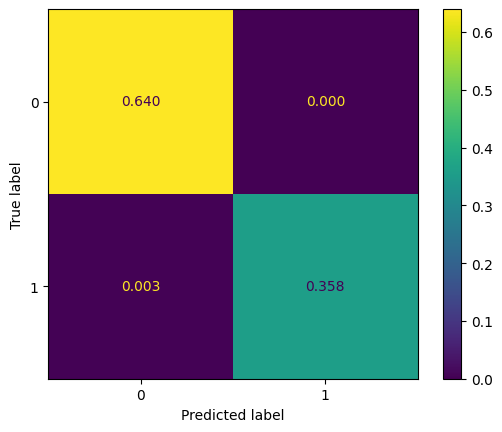
\includegraphics[width=0.5\textwidth]{Pz/MCLP.png}
    \caption{Matriz de Confusión promedio de los conjuntos de prueba asociada al SVM (Modelo A) con kernel ``linear''.}
    \label{fig:1}
\end{figure}
Para el conjunto con el kernel lineal, el modelo predijo un 64.0 \% de coincidencia  para los valores de 0 y un 35.8\% para los valores de 1 teniendo un error en las predicciones de 0.3 \%.
\begin{figure}[H]
    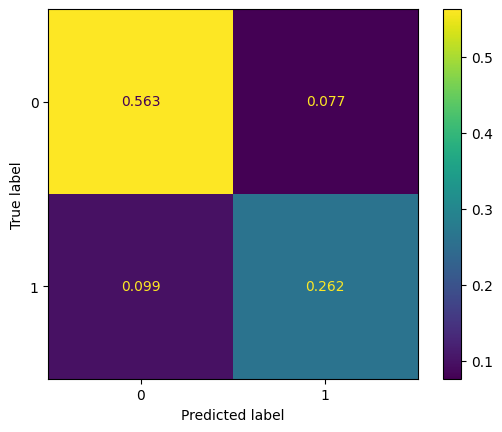
\includegraphics[width=0.5\textwidth]{Pz/MC2P.png}
    \caption{Matriz de Confusión promedio de los conjuntos de prueba asociada al SVM (Modelo A) con kernel ``poly'' de grado 2.}
    \label{fig:2}
\end{figure}
Para el conjunto del kernel polinomial de grado 2, el modelo predijo en 56.3 \% la coincidencia  para los valores de 0 y en 26.2 \% para los valores de 1 teniendo un error en las predicciones de 17.6\%.
\begin{figure}[H]
    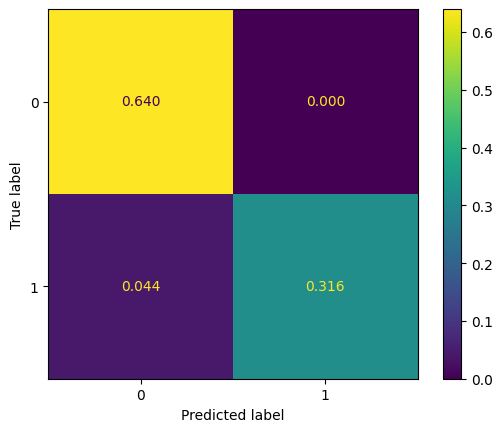
\includegraphics[width=0.5\textwidth]{Pz/MC3P.png}
    \caption{Matriz de Confusión promedio de los conjuntos de prueba asociada al SVM (Modelo A) con kernel ``poly'' de grado 3.}
    \label{fig:3}
\end{figure}
Para el conjunto del kernel polinomial de grado 3, el modelo predijo en 64.0 \% la coincidencia  para los valores de 0 y en 31.6 \% para los valores de 1 teniendo un error en las predicciones de 4.4\%.
\begin{figure}[H]
    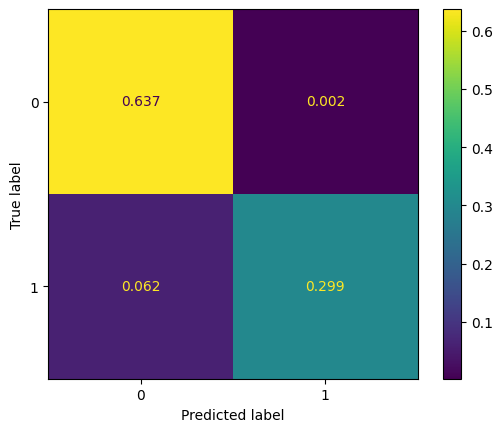
\includegraphics[width=0.5\textwidth]{Pz/MCrP.png}
    \caption{Matriz de Confusión promedio de los conjuntos de prueba asociada al SVM (Modelo A) con kernel ``rbf'' con $\gamma=1$.}
    \label{fig:4}
\end{figure}
Para el conjunto del kernel rbf, el modelo predijo un 63.7 \% de coincidencia  para los valores de 0 y en 29.9 \% para los valores de 1 teniendo un error en las predicciones de 6.2 \%.

Los modelos que mejor lograron predecir los valores del conjunto de datos A correctamente  fueron los que utilizaron los kernel lineal y polinómico de grado 3 con precisiones superiores al 95 \%. EL modelo rbf  también obtuvo valores buenos de predicción con un 93.6 \%.

\subsubsection{Modelos B}
De manera análoga a los modelos A con SVM, se aplicó el conjunto de entrenamiento a los modelos B que se describió en la sección anterior, lo cual permitió obtener las matrices de confusión promedio para los conjuntos de prueba que se ilustran en las figuras \ref{fig:5}, \ref{fig:6}, \ref{fig:7} y \ref{fig:8}.
\begin{figure}[H]
    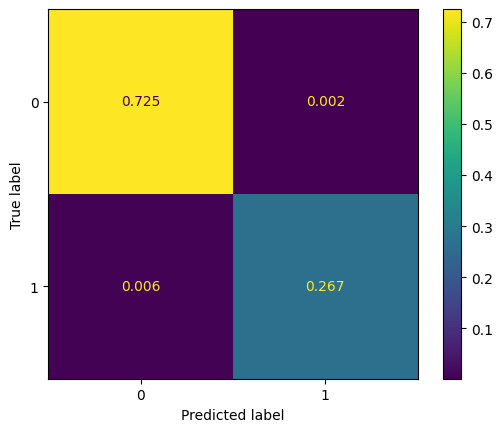
\includegraphics[width=0.5\textwidth]{P/MCLP.png}
    \caption{Matriz de Confusión promedio de los conjuntos de prueba asociada al SVM (Modelo B) con kernel ``linear''.}
    \label{fig:5}
\end{figure}
Para el conjunto con el kernel lineal, el modelo predijo un 72.5 \% de coincidencia  para los valores de 0 y un 26.7 \% para los valores de 1 teniendo un error en las predicciones de 0.8 \%.
\begin{figure}[H]
    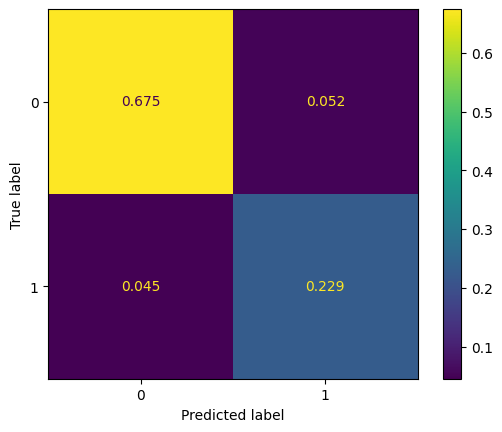
\includegraphics[width=0.5\textwidth]{P/MC2P.png}
    \caption{Matriz de Confusión promedio de los conjuntos de prueba asociada al SVM (Modelo B) con kernel ``poly'' de grado 2.}
    \label{fig:6}
\end{figure}
Para el conjunto del kernel polinomial de grado 2, el modelo predijo en 67.5 \% la coincidencia  para los valores de 0 y en 22.9 \% para los valores de 1 teniendo un error en las predicciones de 9.7 \%.
\begin{figure}[H]
    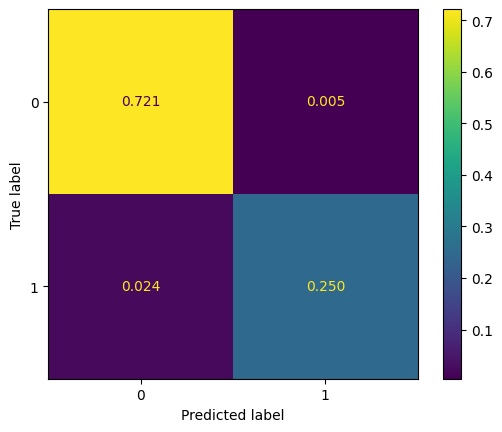
\includegraphics[width=0.5\textwidth]{P/MC3P.png}
    \caption{Matriz de Confusión promedio de los conjuntos de prueba asociada al SVM (Modelo B) con kernel ``poly'' de grado 3.}
    \label{fig:7}
\end{figure}
Para el conjunto del kernel polinomial de grado 3, el modelo predijo en 72.1 \% la coincidencia  para los valores de 0 y en 25.0 \% para los valores de 1 teniendo un error en las predicciones de 2.9\%.
\begin{figure}[H]
    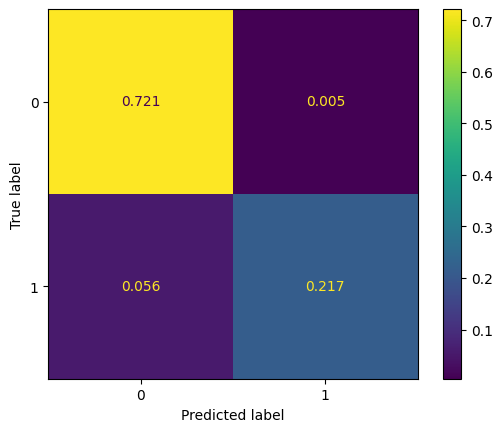
\includegraphics[width=0.5\textwidth]{P/MCrP.png}
    \caption{Matriz de Confusión promedio de los conjuntos de prueba asociada al SVM (Modelo B) con kernel ``rbf'' con $\gamma=1$.}
    \label{fig:8}
\end{figure}
Para el conjunto del kernel rbf, el modelo predijo un 72.1 \% de coincidencia  para los valores de 0 y en 21.7 \% para los valores de 1 teniendo un error en las predicciones de 6.2 \%.

En este caso los modelos que mejor lograron predecir los valores del conjunto de datos A correctamente  fueron los que utilizaron los kernel lineal, polinómico de grado 3 y el rbf con precisiones superiores al 93 \%.
\subsubsection{Modelos C}
Siguiendo la misma metodología aplicada en los modelos A y B se construyeron las matrices de confusión promedio asociadas a los conjuntos de prueba de la base de datos de los modelos C que se aprecian en las figuras \ref{fig:9}, \ref{fig:10}, \ref{fig:11} y \ref{fig:12}.
\begin{figure}[H]
    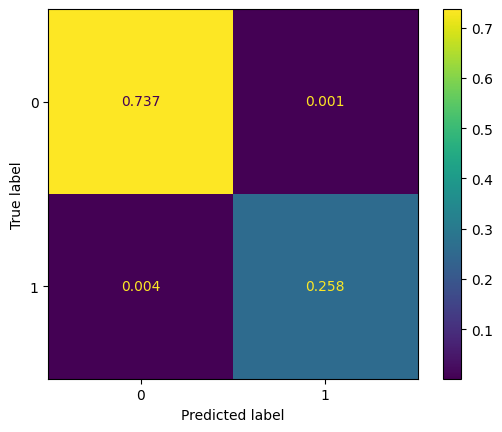
\includegraphics[width=0.5\textwidth]{NoPz/MCLP.png}
    \caption{Matriz de Confusión promedio de los conjuntos de prueba asociada al SVM (Modelo C) con kernel ``linear''.}
    \label{fig:9}
\end{figure}
EL kernel lineal obtuvo un porcentaje de aciertos para los valores de 0 y 1 del 73.7 \% y 25.8\% respectivamente. El error del modelo en las predicciones fue de 0.5 \%.
\begin{figure}[H]
    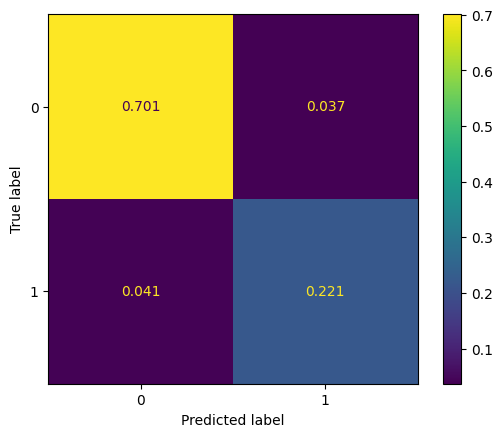
\includegraphics[width=0.5\textwidth]{NoPz/MC2P.png}
    \caption{Matriz de Confusión promedio de los conjuntos de prueba asociada al SVM (Modelo C) con kernel ``poly'' de grado 2.}
    \label{fig:10}
\end{figure}
El kernel polinomial de grado 2 predijo en un 70.1\% de coincidencia los valores de 0 y en 22.1 \%  los valores de 1 teniendo un error en las predicciones del 7.8 \%.
\begin{figure}[H]
    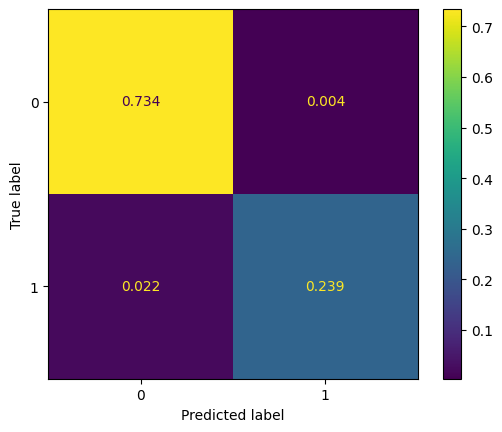
\includegraphics[width=0.5\textwidth]{NoPz/MC3P.png}
    \caption{Matriz de Confusión promedio de los conjuntos de prueba asociada al SVM (Modelo C) con kernel ``poly'' de grado 3.}
    \label{fig:11}
\end{figure}
Para el conjunto del kernel polinomial de grado 3, el modelo predijo en 73.4 \% la coincidencia  para los valores de 0 y en 23.9 \% para los valores de 1 teniendo un error en las predicciones de 2.6 \%.
\begin{figure}[H]
    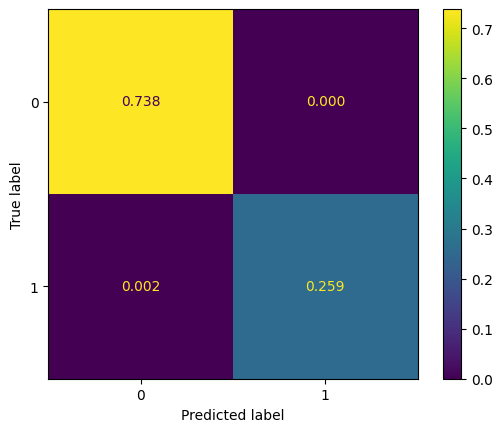
\includegraphics[width=0.5\textwidth]{NoPz/MCrP.png}
    \caption{Matriz de Confusión promedio de los conjuntos de prueba asociada al SVM (Modelo C) con kernel ``rbf'' con $\gamma=1$.}
    \label{fig:12}
\end{figure}
Para el conjunto del kernel rbf, el modelo predijo un 73.8 \% de coincidencia  para los valores de 0 y en 25.9 \% para los valores de 1 teniendo un error en las predicciones de 0.2 \%.

En este caso los modelos que mejor lograron predecir los valores del conjunto de datos A correctamente  fueron los que utilizaron los kernel lineal y el rbf con precisiones superiores al 99 \%

La tabla \ref{tab:my_label1} resume la información obtenida de los distintos algoritmos SVM utilizados para los conjuntos de datos descritos:

De acuerdo a los resultados obtenidos se evidencia que  en general todos los algoritmos tienen buenos resultados en las predicciones con los distintos conjuntos, sin embargo el método que usa el kernel polinómico de grado 2 presenta resultados ligeramente mas bajos de predicción respecto a los demás, con una media de aciertos de 88.4 \%. El método que mejor logra predecir  la clasificación de los datos es el que uso el kernel lineal por lo que se infiere que dadas las características de importancia usadas para la correlación en los distintos conjuntos de datos, la clasificación o coincidencia puede ser descrita mejor con un modelo lineal.

\begin{table}
    \centering
    \scalebox{0.8}{\begin{tabular}{|lllllll|} \hline
    \rowcolor[HTML]{EFEFEF}
        & Modelo A &     & Modelo B &     & Modelo C &  \\ \hline
    \multicolumn{1}{|p{5.355em}}{Algoritmo (Kernel)} & \multicolumn{1}{p{4.355em}}{acertados (\%)} & \multicolumn{1}{p{4.355em}}{erróneos (\%)} & \multicolumn{1}{p{4.355em}}{acertados (\%)s} & \multicolumn{1}{p{4.355em}}{erróneos (\%)} & \multicolumn{1}{p{4.355em}}{acertados (\%)s} & \multicolumn{1}{p{4.355em}|}{erróneos (\%)} \\ \hline
    Linear & 99.8 & 0.3 & 99.2 & 0.8 & 99.5 & 0.5 \\ \hline
    Poly Gr 2 & 82.5 & 17.6 & 90.4 & 9.7 & 92.2 & 7.8 \\ \hline
    Poly Gr3 & 95.6 & 4.4 & 97.1 & 2.9 & 97.3 & 2.6 \\ \hline
    rbf & 93.6 & 6.4 & 93.8 & 6.1 & 99.7 & 0.2 \\ \hline
    \end{tabular}}
    \caption{Comparación de los resultados de predicción del método SVM, por tipo de algoritmo y conjunto de datos según las matrices de confusión.}
    \label{tab:my_label1}
\end{table}
\subsection{Regresión Logística}
El algoritmo de regresión logística presentó puntajes de validación relativamente altos para todos los modelos. El Modelo C obtuvo un valor de 99.34\%, el Modelo B 98.40\% y el Modelo A, que considera todos los parámetros de entrenamiento, mostró un score de validación de 99.07\%, el más alto de todos. Esto es debido a la naturaleza de la regresión logística que es adecuada para la clasificación binaria a través de la función sigmoide. En la tabla \ref{tab:my_label2} se muestra el resumen del rendimiento de este algoritmo para los tres modelos.

\begin{table}
    \centering
    \begin{tabular}{|c|c|} \hline
    \rowcolor[HTML]{EFEFEF}
         Modelo & Validation Score \\ \hline
         A & 99.07\% \\ \hline
         B & 98.40\%\\ \hline
         C & 99.34\%\\ \hline
    \end{tabular}
    \caption{Puntajes de validación de la Regresión Logística para los tres modelos}
    \label{tab:my_label2}
\end{table}
En las figuras \ref{fig:13}, \ref{fig:14} y \ref{fig:15} se muestran las matrices de confusión de la regresión logística para los modelos A, B y C respectivamente.
\begin{figure}
    \centering
    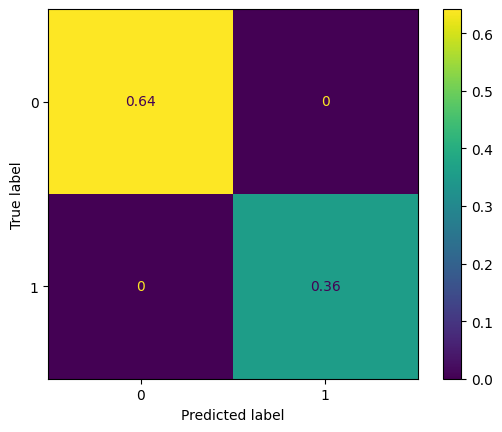
\includegraphics[width=0.5\textwidth]{reg logistica/reglogPz.png}
    \caption{Matriz de confusión de la regresión logística del modelo A}
    \label{fig:13}
\end{figure}

\begin{figure}
    \centering
    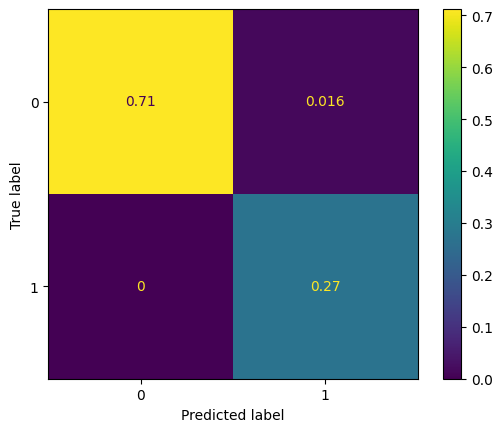
\includegraphics[width=0.5\textwidth]{reg logistica/reglogP.png}
    \caption{Matriz de confusión de la regresión logística del modelo B}
    \label{fig:14}
\end{figure}

\begin{figure}
    \centering
    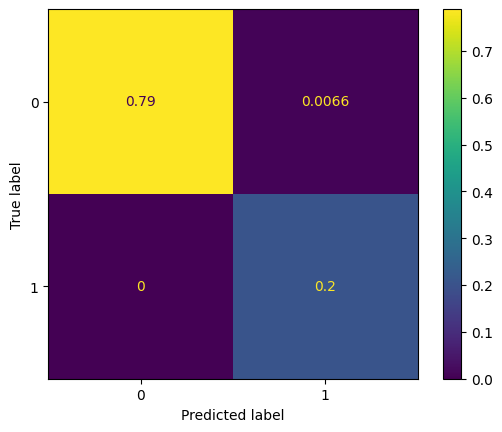
\includegraphics[width=0.5\textwidth]{reg logistica/reglog.png}
    \caption{Matriz de confusión de la regresión logística del modelo C}
    \label{fig:15}
\end{figure}

\subsection{Redes Neuronales}
Los rendimientos de todas las redes neuronales probadas fueron similares para todos los modelos. Para el Modelo C, se obtuvo una precisión superior al 98.68\%  con todas las redes tanto para los conjuntos de entrenamiento como de prueba, con valores de las funciones de pérdida del orden de entre $10^-8$ y $10^-6$. Una de las curvas de la función de pérdida se muestra en la figura \ref{fig:16}.
\begin{figure}[H]
    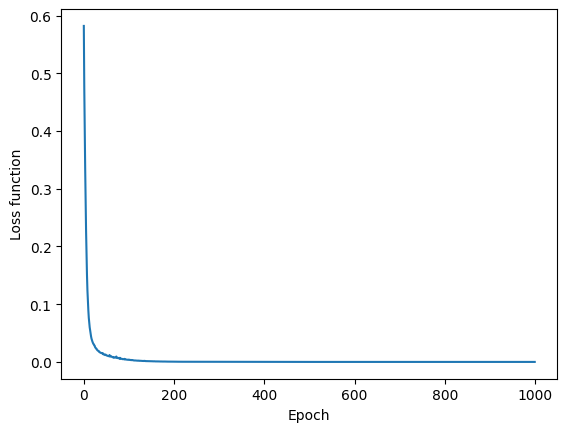
\includegraphics[width=0.5\textwidth]{redes/loss.png}
    \caption{Curva de función de pérdida por época de entrenamiento}
    \label{fig:16}
\end{figure}
Para el Modelo B se obtuvo una precisión superior al 96.80\% en los dos esquemas de redes. Para el Modelo A, que toma en cuenta todos los parámetros de la tabla \ref{tab:my_label}, se obtuvo una precisión superior al 97.53\%, que es ligeramente mejor que para el Modelo B. Esto implica que el redshift es una característica relevante para la predicción de las coincidencias. De haber contado con una mayor cantidad de datos con este parámetro, como en el caso del Modelo C, se esperaría que la precisión del modelo sea incluso mayor a la obtenida con el modelo C.
En la tabla \ref{tab:my_label2} se muestra el resumen de las precisiones alcanzadas por las redes neuronales para cada modelo.

\begin{table}
    \centering
    \scalebox{0.8}{\begin{tabular}{|lllllll|} \hline
    \rowcolor[HTML]{EFEFEF}
        & Modelo A &     & Modelo B &     & Modelo C &  \\ \hline
    \multicolumn{1}{|p{5.355em}}{Red Neuronal} & \multicolumn{1}{p{4.355em}}{épocas} & \multicolumn{1}{p{4.355em}}{precisión (\%)} & \multicolumn{1}{p{4.355em}}{épocas} & \multicolumn{1}{p{4.355em}}{precisión (\%)} & \multicolumn{1}{p{4.355em}}{épocas} & \multicolumn{1}{p{4.355em}|}{precisión (\%)} \\ \hline
    Esquema 1 & 1000 & 100 & 1000 & 100 & 1000 & 100 \\ \hline
    Esquema 2 & 50 & 97.53 & 50 & 96.80 & 50 & 98.68 \\ \hline
    \end{tabular}}
    \caption{Precisión de las redes neuronales para los tres modelos por número de épocas de entrenamiento.}
    \label{tab:my_label2}
\end{table}
\subsection{Red Neuronal Convolucional}
Como ya se mencionó, la cantidad reducida de datos disponible para entrenar esta red no permitió obtener un rendimiento sobresaliente. Se obtuvo un valor promedio para la métrica "mse" de 1.98, que se puede considerar aceptable, tomando en cuenta este problema además de los errores en las mediciones de la magnitud en B al comparar los dos catálogos. En la tabla \ref{tab:my_label3} se muestran algunos ejemplos de las predicciones realizadas para los objetos del conjunto de datos de predicciones.

\begin{table}
    \centering
    \begin{tabular}{|c|c|c|} \hline
    \rowcolor[HTML]{EFEFEF}
         AT20G ObjID & Magnitud B Real & Magnitud B predicha \\ \hline
         257 & 20.424 & 20.206 \\ \hline
         258 & 18.875 & 18.915 \\ \hline
         259 & 18.183 & 18.830 \\ \hline
         260 & 18.851 & 18.580 \\ \hline
         261 & 17.906 & 17.910 \\ \hline
    \end{tabular}
    \caption{Magnitudes en B reales y predichas por la CNN para 4 objetos de prueba del catálogo AT20G}
    \label{tab:my_label3}
\end{table}

La Figura 17 muestra algunas de las imágenes de los objetos de las predicciones mostradas en la tabla \ref{tab:my_label3}.
\begin{figure}
    \centering
    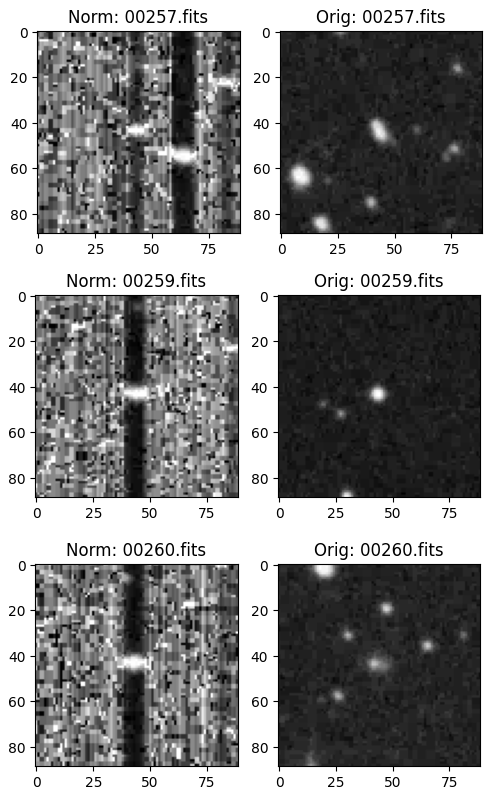
\includegraphics[width=0.5\textwidth]{redes/cnn.png}
    \caption{Imágenes en filtro B de tres objetos del catálogo AT20G obtenidas en SuperCosmos. Normalizadas (izquierda), Originales (derecha)}
    \label{fig:17}
\end{figure}

\subsection{Predicciones}
Para determinar las predicciones correctas entre los dos catálogos se tomaron los resultados positivos (1) de cada algoritmo y se estableció como criterio de "match" aquellos registros que más algoritmos con valor 1 en la columna de coincidencia presentaban para cada objeto del AT20G relacionado con un objeto de SuperCosmos, es decir  se considero como un valor de acierto aquel en el que en la mayoría de algoritmos se presentaba como una  con valor de 1. De esta manera, efectivamente, se encontró una sola coincidencia para cada objeto. Este proceso se hizo para cada modelo. Luego, las coincidencias finales se establecieron a partir de la unión de los resultados de coincidencias de los tres modelos. Se pudo determinar que si un objeto presentaba coincidencia positiva en el Modelo C que es el que menos parámetros de entrenamiento utiliza, también presentaba coincidencia en los Modelos A y B que utilizan dos y un parámetro adicional respectivamente. Finalmente, si para un mismo objeto del AT20G se tenían dos coincidencias positivas, que fue el máximo número de coincidencias simultáneas, se seleccionó la que primero aparece en la tabla de coincidencias. Esto debido a que los objetos se encuentran ordenados en función de la separación entre las coordenadas de radio y óptico, y este parámetro es uno de los más relevantes en el crossmatching.

En la Tabla VI se presenta una muestra de las coincidencias de objetos con coincidencia y sin coincidencia encontrada tomando en cuenta los tres modelos. Además, se indica un objeto para el cual se encontró más de una coincidencia simultánea.
\begin{table}
    \centering
    \begin{tabular}{|c|c|c|c|c|c|} \hline
    \rowcolor[HTML]{EFEFEF}
        ObjID AT20G & Bmag SC & A & B & C & Coincidencia \\ \hline
         5 & \textbf{20.023} & 1 & 1 & 1 & 1\\  \hline
         5 & 21.073 & 0 & 0 & 0 & 0\\  \hline
         5 & 21.963 & 0 & 0 & 0 & 0\\  \hline
         20 & \textbf{17.844} & 1 & -- & -- & 1\\  \hline
         20 & 21.205 & 0 & -- & 0 & 0\\  \hline
         84 & 16.9 & 0 & 0 & -- & 0 \\  \hline
         84 & 16.9 & 0 & 0 & -- & 0 \\  \hline
         104 & \textbf{20.187} & 1 & 1 & -- & 1\\  \hline
         104 & 22.056 & 1 & 1 & -- & 1\\  \hline
         312 & \textbf{19.187} & 1 & 1 & 1 & 1\\  \hline
    \end{tabular}
    \caption{Ejemplos de selección de coincidencias positivas para objetos del AT20G con SuperCosmos. Nota: las entradas vacías indican que para ese registro no se disponía del valor de P20 y/o redshift. Los valores en negrita indican el valor de la magnitud B del objeto de SuperCosmos. Para el objeto con ID 84, por ejemplo, no se encontró coincidencia.}
    \label{tab:my_label4}
\end{table}
Una vez determinadas las coincidencias, se realizó la validación de las mismas, utilizando el programa Aladin. Se ingresaron las coordenadas de radio del objeto y las de óptico de SuperCosmos y se verificó si había la detección del objeto en el radio que contiene las dos coordenadas. De esta manera se lograron encontrar 78 nuevas coincidencias de los 91 objetos sin identificar del catálogo AT20G. En la figura 18 se presenta una muestra de las coincidencias encontradas para cuatro objetos del AT20G.
\begin{figure}
    \centering
    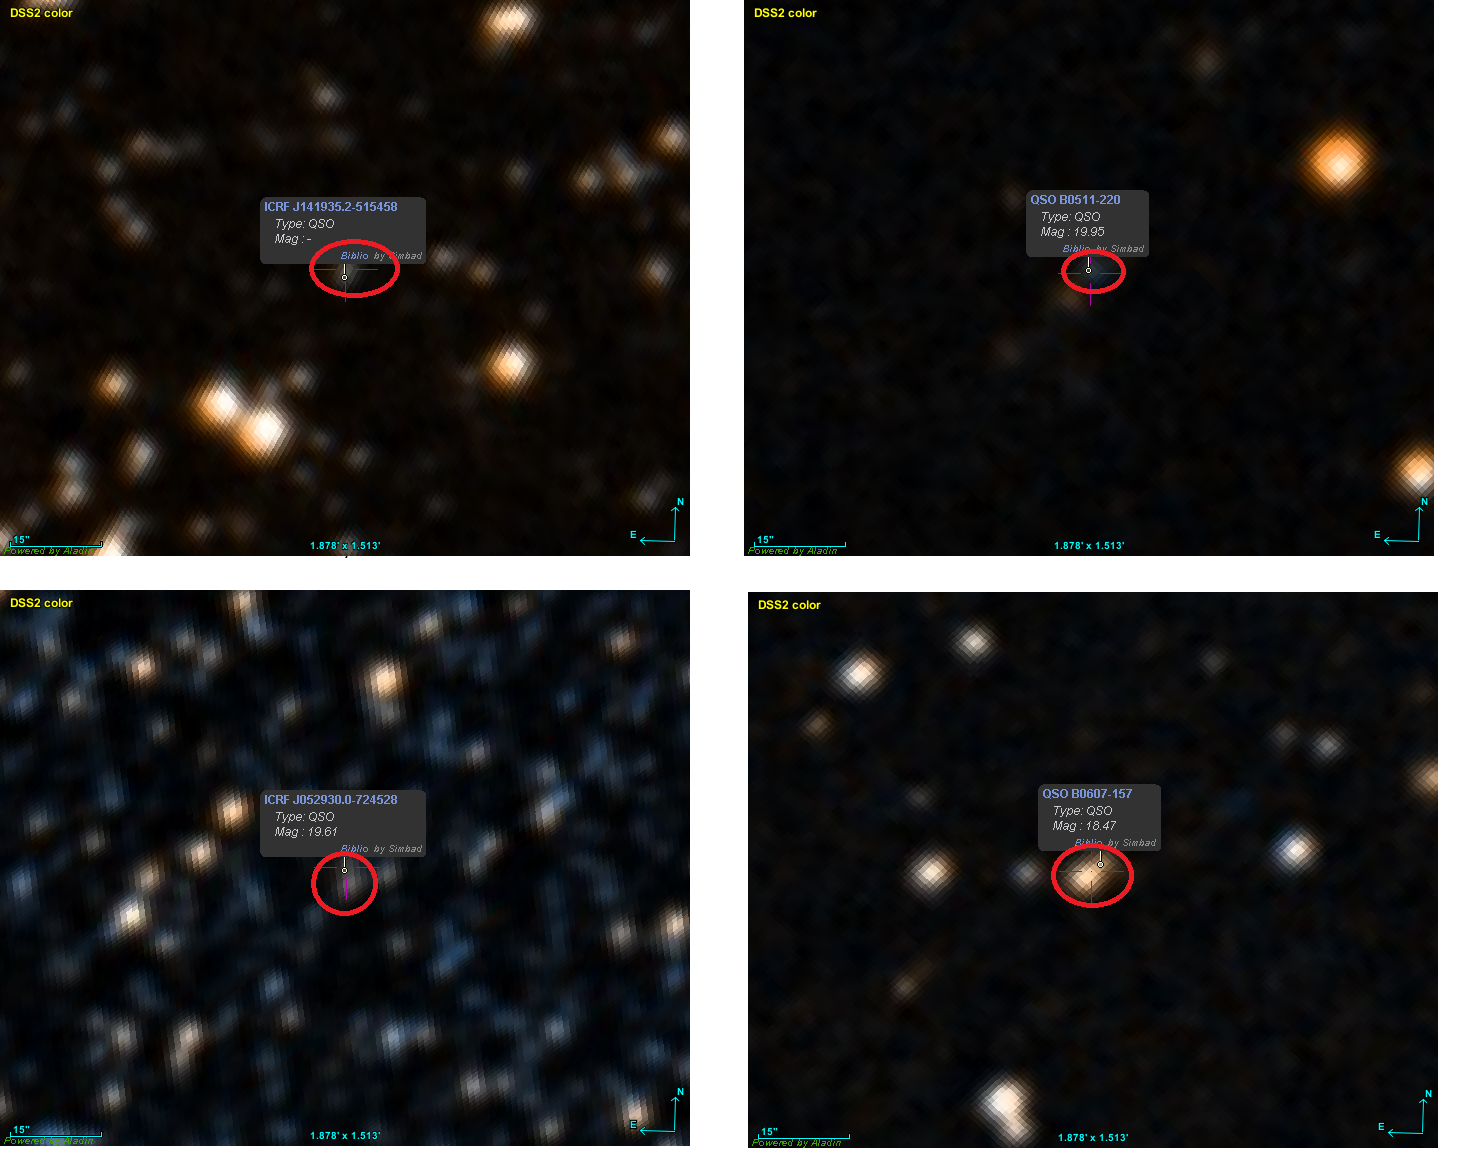
\includegraphics[width=0.5\textwidth]{redes/matches.png}
    \caption{Coincidencias encontradas para cuatro objetos del AT20G con ObjIDs: 5 y 66 (Arriba). 73 y 83 (abajo).}
    \label{fig:18}
\end{figure}

 

\section{Conclusiones}
Este proyecto de crossmatching astronómico demostró la utilidad de aplicar diferentes algoritmos de aprendizaje automático en identificar coincidencias de objetos entre catálogos astronómicos, esta metodología tiene importantes implicaciones para la investigación astronómica al proporcionar información valiosa sobre objetos celestes previamente no identificados en el espacio radio y óptico, haciendo que la información disponible sea complementada o completada.

Se observó que los algoritmos trabajan mejor con una mayor cantidad de datos y más parámetros relevantes. Particularmente, cuando se trabajó con el redshift (Modelo A) se obtuvieron valores de precisión más altos aunque se disponía de menos datos.

Aunque los algoritmos implementados presentan diferencias en su estructura y forma de trabajo, todos mostraron rendimientos altos, con valores de precisión superiores al 95\%.

En las redes neuronales, se implementaron estructuras relativamente simples, que, con un número pequeño de épocas de entrenamiento lograron alcanzar precisiones mayores al 98\%. 
Al tratar al problema como uno de clasificación binaria, para el caso de las redes neuronales se pudo utilizar distintas opciones en las funciones de activación de las capas de salida como la softmax, para un problema de dos clases con valores enteros, y la sigmoide para uno de clasificación binaria.
\newpage
\printbibliography[title={Referencias}]
\end{document}
